\documentclass{article}

\usepackage{microtype}
\usepackage{amsmath}
\usepackage{enumitem}
\usepackage{etoolbox}
% \usepackage{pgfplots}
\usepackage[svgnames]{xcolor}
\usepackage{tikz}
\usepackage{tikz-3dplot}
\usepackage[letterpaper, bottom=100pt]{geometry}
\usepackage{physics}
\usepackage{MnSymbol}
\usepackage{float}

% \pgfplotsset{compat=newest}

\newcommand{\diff}[1]{\frac{#1}{dt}}
\newcommand{\vel}{\mathrm{v}}
\newcommand{\x}{\mathrm{x}}
\newcommand{\inter}{\int_{t_1}^{t_2}}
\newcommand{\tvert}{\biggr\rvert_{t_1}^{t_2}}
\newcommand{\derv}{\frac{\mathrm{d}}{\mathrm{d}t}}

\patchcmd\subequations
 {\theparentequation\alph{equation}}
 {\subequationsformat}
 {}{}

\newcommand{\subequationsformat}{\theparentequation.\arabic{equation}}

\author{Laith}
\title{Constant Acceleration Textbook Problems}
\date{1/30/2023}

\begin{document}
\maketitle
\section{$\bigstar$Problem 23}
An electron with an initial velocity $v_0=1.50\times10^5\,\mathrm{m/s}$
enters a region of length $L=1.00\,\mathrm{cm}$ where it is electrically
accelerated. It emerges with $v=5.70\times10^6\,\mathrm{m/s}$. What is
its acceleration, assumed constant?
\begin{figure}[H]
    \begin{center}
        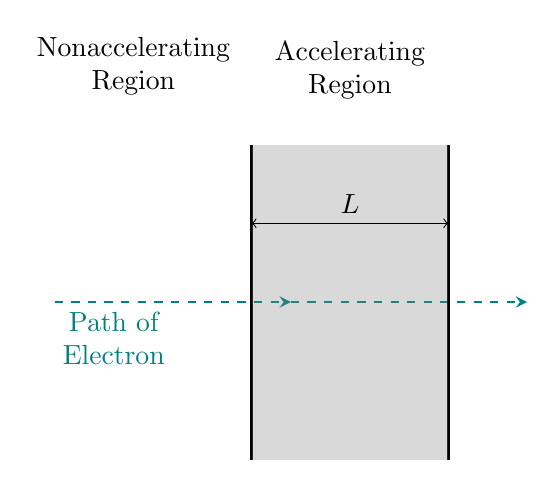
\begin{tikzpicture}[every text node part/.style={align=center}]
            \node at (1, 3) {Nonaccelerating\\Region};

            \draw[thick, line width=1pt] (2.5, 0) coordinate (a) -- (2.5, 2) coordinate (d);
            \draw[thick, line width=1pt] (a) -- (2.5, -2) coordinate (d2);

            \draw[-stealth, dashed, thick, color=teal] (0, 0) -- (3, 0) node[near start, below] (p) {Path of \\Electron};
            \draw[-stealth, dashed, thick, color=teal] (3, 0) -- (6, 0);

            \draw[thick, line width=1pt] (5, 0) coordinate (b) -- (5, -2) coordinate (c2);
            \draw[thick, line width=1pt] (b) -- (5, 2) coordinate (c); 

            \fill[color=gray, opacity=0.3] (a) -- (b) -- (c) -- (d);
            \fill[color=gray, opacity=0.3] (a) -- (b) -- (c2) -- (d2);

            \draw[<->] (2.5, 1) -- (5, 1) node[above, midway] (l) {$L$};
            \node[above of = l, yshift=20] {Accelerating\\Region};
        \end{tikzpicture} 
    \end{center}
\end{figure}

\subsection{Solution}
We have an initial velocity $v_0=1.50\times10^5\,\mathrm{m/s}$, final velocity $v=5.70\times10^6\,\mathrm{m/s}$, 
and distance $L=1.00\,\mathrm{cm}$. We could use the below formula:
\[v^2=v_0^2+2a(x-x_0)\]
Since we already have $v$ and $v_0$ as well as $x$ and $x_0$, all we need to do is isolate acceleration:
\begin{subequations}
    \begin{align}
        v^2 &= v^2_0+2a(x-x_0) \\
        \Rightarrow v^2-v^2_0 &= 2a(x-x_0) \\
        \Rightarrow \frac{1}{2}(v^2-v^2_0) &= a(x-x_0) \\
        \Rightarrow \frac{\frac{1}{2}(v^2-v^2_0)}{x-x_0} &= a \\
        a &= \frac{(v^2-v^2_0)}{2(x-x_0)}
    \end{align}
    
Before we substitue in our values, we need to convert our distance from cm to m in order to
keep our units consistent and thus our answer correct:
\[L=1.00\,\mathrm{cm}\times\frac{1\,\mathrm{m}}{100\,\mathrm{cm}}=0.01\,\mathrm{m}\]
Now to substitute in our values:
\begin{align}
    a &= \frac{((5.7\times10^6)^2-(1.5\times10^5)^2)}{2(0.01-0)} \\
    a &= \frac{((5.7^2\times10^{6\times2})-(1.5^2\times10^{5\times2}))}{2(0.01)} \\
    a &= \frac{((32.5\times10^{12})-(2.25\times10^{10}))}{0.02} \\
    a &= \frac{10^{10}(32.5\times10^{2}-2.25)}{0.02} \\
    a &= \frac{10^{10}(3250-2.25)}{0.02} \\
    a &= \frac{10^{10}(3247.75)}{0.02} \\
    a &= \frac{10^{10}(3.24775\times10^3)}{0.02} \\
    a &= \frac{(3.24775\times10^{13})}{0.02} \\
    a &= 162.3875\times10^{13} \\
    a &= 1.623875\times10^{15} \\
    a &= 1.624\times10^{15}
\end{align}
\end{subequations}
\newpage
\section{$\bigstar$ Problem 24}
\emph{Catapulting mushrooms.} Certain mushrooms launch
their spores by a catapult mechanism. As water condenses from
the air onto a spore that is attached to the mushroom, a drop grows
on one side of the spore and a film grows on the other side. The
spore is bent over by the drop’s weight, but when the film reaches
the drop, the drop’s water suddenly spreads into the film and the
spore springs upward so rapidly that it is slung off into the air. Typically, 
the spore reaches a speed of $1.6\,\mathrm{m/s}$ in a $5.0\,\mathrm{\mu m}$ launch; 
its speed is then reduced to zero in $1.0\,\mathrm{mm}$ by the air. Using those data
and assuming constant accelerations, find the acceleration in terms
of g during (a) the launch and (b) the speed reduction.

\subsection{Solution}
We can draw the scenario:
\begin{figure}[H]
    \begin{center}
        \begin{tikzpicture}[every text node part/.style={align=left}]
            \coordinate (a) at (2, 0);
            \coordinate (b) at (2, 1);
            \coordinate (c) at (2, 4);

            \draw (0, 0) node[left] {$v_0=0\,\mathrm{m/s}$\\$x_0=0\,\mathrm{m}$} -- (4, 0);
            \draw[dashed, -stealth] (a) 
            -- (b) node[blue, scale=3] {.} node[right] {$v_1=1.6\,\mathrm{m/s}$\\$x_2=5.0\,\mathrm{\mu m}$} 
            -- (c) node[red, scale=3] {.} node[right] {$v_2=0\,\mathrm{m/s}$\\$x_1=1.0\,\mathrm{mm}$};
        \end{tikzpicture}
    \end{center}
\end{figure}

We need to find the acceleration from the ground to the blue point and then the acceleration from the
blue point to the red point, both in terms of gravity g. Since we have values for velocity and position,
we can use this formula:
\[v^2 = v^2_0+2a(x-x_0) \Rightarrow a = \frac{v^2-v^2_0}{2(x-x_0)}\]
For the first acceleration:
\begin{subequations}
    \begin{subequations}
        
    \begin{align}
        v = 1.6 \,\mathrm{m/s} \\
        v_0 = 0 \,\mathrm{m/s} \\
        x = 5.0 \,\mathrm{\mu m} = 5.0\cdot10^{-6} \,\mathrm{m} \\
        x_0 = 0 \,\mathrm{\mu m} \\
        a &= \frac{(1.6)^2-(0^2)}{2(5.0\cdot10^{-6}-0)} \\
          &= \frac{1.6^2}{2(5.0\cdot10^{-6})} \\
          &= \frac{2.56}{10\cdot10^{-6}} \\
          &= \frac{2.56}{10^{-5}} \\
        a &= 2.56\cdot10^{5} \,\mathrm{m/s^2}
    \end{align}
Now to write this in terms of gravity, we divide this value by $g=9.8\,\mathrm{m/s^2}$.
\begin{align}
    a &= 2.56\cdot10^5 \,\mathrm{m/s^2} \cdot \frac{g}{9.8\,\mathrm{m/s^2}} \\
    a &= \frac{2.56\cdot10^5}{9.8}g \\
    a &= 2.61\cdot10^4g
\end{align}
\end{subequations}

For the second acceleration:
\begin{subequations}
\begin{align}
    v = 0 \,\mathrm{m/s} \\
    v_0 = 1.6 \,\mathrm{m/s} \\
    x = 1.0 \,\mathrm{mm} = 1.0\cdot10^{-3}\,\mathrm{m} \\
    x_0 = 5.0\cdot10^{-5} \,\mathrm{m} \\
    a &= \frac{(0)^2-(1.6^2)}{2(1.0\cdot10^{-3}-5.0\cdot10^{-5})} \\
      &= \frac{-(1.6^2)}{2\cdot10^{-3}(1.0-5.0\cdot10^{-2})} \\
      &= \frac{-2.56}{2\cdot10^{-3}(0.95)} \\
      &= \frac{-2.56}{0.0019} \\
    a &= -1.347\cdot10^3 \,\mathrm{m/s^2} \\
    \text{\textbf{In terms of gravity:}  } 
    a &= \frac{-1.347\cdot10^3}{9.8}g \\
    a &= -1.37\cdot10^2g
\end{align}
\end{subequations}
\end{subequations}
    
\end{document}